\section{Benchmarkdatensatz} \label{sec:Benchmarkdatensatz}

Die zu implementierenden Metaheuristiken und proaktiven, prädiktiven und reaktiven Verfahren gilt es auf eine gemeinsame Datenbasis für das \ac{mrcpsp} zu validieren. Unzählige wissenschaftliche Arbeiten, wie die von \cite{rezaeian_using_2015}, \cite{jozefowska_simulated_2001} oder \cite{al-fawzan_bi-objective_2005} nutzen zur Evaluierung ihrer Ergebnisse für das \ac{mrcpsp} die PSPLIB von \cite{kolisch_psplib_1997}. Dort enthalten sind Instanzsets, welche neben unterschiedlich generierten Projektplänen auch die Informationen zu den minimalen Projektdauern beinhalten. 

\begin{table}[H]
\centering
\begin{tabular}{r|ccccc}
& m1  & m2  & n0  & n1  & j20 \\ \hline
Instanzen & 640 & 481 & 470 & 637 & 554 \\ \hline
Aktivitäten & 16  & 16  & 10  & 16  & 20  \\
Modi & 1   & 2   & 3   & 3   & 3   \\ \hline
Erneuerbare Ressourcenarten & 2   & 2   & 2   & 2   & 2   \\
Nicht erneuerbare Ressourcenarten & 2   & 2   & 0   & 1   & 2  
\end{tabular}

\caption{Metadaten zu den verwendeten Instanzsets der PSPLIB \cite{kolisch_psplib_1997}}
\label{tab:instanzsets}
\source{Eigene Darstellung}
\end{table}

Tabelle \ref{tab:instanzsets} repräsentiert fünf Instanzsets der PSPLIB von \cite{kolisch_psplib_1997}. Im Rahmen der Evaluierung werden diese verwendet, um die Metaheuristiken miteinander vergleichen zu können. Durch die unterschiedlichen Anzahlen von Aktivitäten, Modi und (nicht) erneuerbaren Ressourcenarten werden die Metaheuristiken mit andersartigen komplexen Gegebenheiten evaluiert. Die PSPLIB beinhaltet zudem das Instanzset j30.mm mit 30 Aktivitäten, in welcher die angegebenen minimalsten Projektdauern zum Zeitpunkt der Masterarbeit nur heuristisch sind, da globale Optima durch die immense Menge an Permutationen nicht bestimmt werden können.\\

Eine konkrete Instanz n01\_2.mm der PSPLIB vom Benchmarkset n0 kann aus Listing \ref{lst:psplib_n0_example} entnommen werden. Einzelne Sektionen zur Beschreibung des Projektplans werden über Sternchen- und Minuszeichen voneinander getrennt. Die ersten drei Sektionen geben Metainformationen, wie die Anzahl der Aktivitäten, Ressourcenarten, maximale Dauer über Horizon, und Daten zur Generierung der Instanz an. Der vierte Bereich zeigt zum einen die Abhängigkeiten der Aktivitäten und zum anderen die Anzahl der möglichen Modi für eine Aktivität auf. Die Modi werden in dem fünften Bereich mit einer Ausführdauer und den Ressourcenanforderungen definiert. Im sechsten und letzten Bereich der Datei werden die für das Projekt verfügbaren Ressourcen aufgeführt. 

\begin{lstlisting}[caption={Instanz n01\_2.mm der PSPLIB n0 (Quelle:  \cite{kolisch_psplib_1997})}, label=lst:psplib_n0_example, basicstyle=\scriptsize, breaklines=true,breakatwhitespace=true, columns=flexible]
************************************************************************
file with basedata            : me1_.bas
initial value random generator: 466396357
************************************************************************
projects                      :  1
jobs (incl. supersource/sink ):  12
horizon                       :  65
RESOURCES
  - renewable                 :  2   R
  - nonrenewable              :  0   N
  - doubly constrained        :  0   D
************************************************************************
PROJECT INFORMATION:
pronr.  #jobs rel.date duedate tardcost  MPM-Time
    1     10      0        8        6        8
************************************************************************
PRECEDENCE RELATIONS:
jobnr.    #modes  #successors   successors
   1        1          3           2   3   4
   2        3          3           5   7   9
   3        3          2           8   9
   4        3          3           5   6   7
   5        3          2          10  11
   6        3          2           8   9
   7        3          2          10  11
   8        3          2          10  11
   9        3          1          12
  10        3          1          12
  11        3          1          12
  12        1          0        
************************************************************************
REQUESTS/DURATIONS:
jobnr. mode duration  R 1  R 2
----------------------------------------
  1      1     0       0    0
  2      1     1       0   10
         2     6       6    0
         3     9       0    8
  3      1     3       4    0
         2     5       0    7
         3     7       0    4
  4      1     1       7    0
         2     5       0   10
         3     8       5    0
  5      1     1       0    5
         2     2       0    4
         3     6       2    0
  6      1     2       0    3
         2     3       8    0
         3     6       7    0
  7      1     6       6    0
         2     8       4    0
         3     9       3    0
  8      1     1      10    0
         2     2       8    0
         3     3       0    6
  9      1     1       7    0
         2     4       6    0
         3     4       0    6
 10      1     1       6    0
         2     1       0    7
         3     3       0    6
 11      1     1       0    3
         2     8       4    0
         3    10       3    0
 12      1     0       0    0
************************************************************************
RESOURCEAVAILABILITIES:
  R 1  R 2
    7    7
************************************************************************
\end{lstlisting}

In Abbildung \ref{img:psplib_n0_example} lässt sich der Projektplan für die Instanz n01\_2.mm grafisch visualisieren. Diese Darstellungsart ist angelehnt an die aus Abbildung \ref{img:example_mrcpsp}.

\begin{figure}[H]
    \centering
    \noindent\makebox[\textwidth]{%
    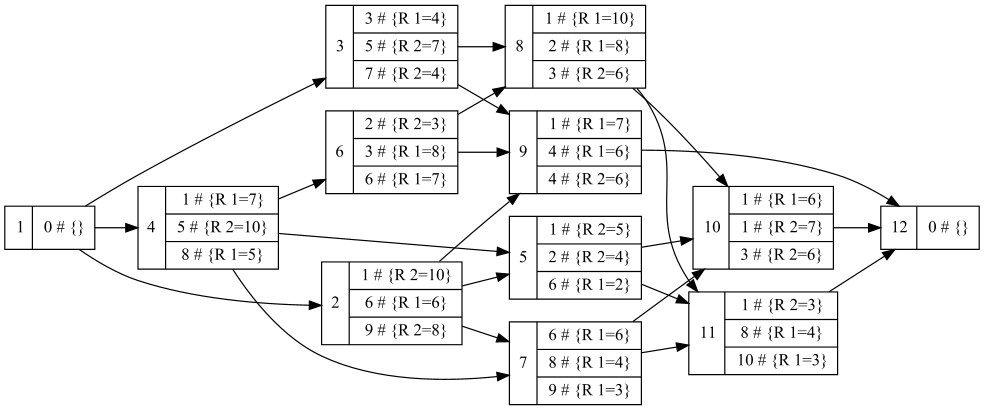
\includegraphics[width=\textwidth]{assets/img/03_Konzept/n01_2.png}
    }
    \caption{Visualisierung des Projektplans der Instanz n01\_2.mm der PSPLIB n0} 
    \label{img:psplib_n0_example}
    \source{Eigene Darstellung}
\end{figure}